\subsection{Протокол Ву~---~Лама}\index{протокол!Ву~---~Лама|(}\label{section-woo-lam}
\selectlanguage{russian}

Протокол Ву~---~Лама, предложенный в 1992 году (\langen{Woo, Lam},~\cite{Woo:Lam:1992:1, Woo:Lam:1992:3}), добавляет к сообщениям случайные числа участников, что позволяет защитить протокол в том числе от атак повтором, а также обеспечивает подтверждение владения ключами. Также это единственный из рассмотренных в этом разделе протоколов, в котором новый ключ формируется доверенной стороной (Трентом).

\begin{figure}
    \centering
    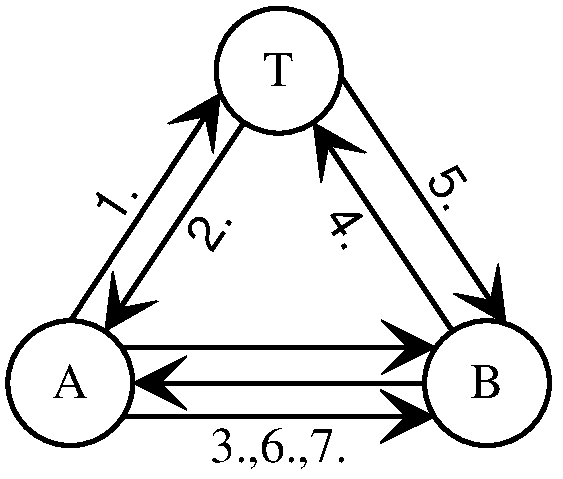
\includegraphics[width=0.5\textwidth]{pic/woo-lam}
    \caption{Взаимодействие участников в протоколе Ву~---~Лама\label{fig:woo-lam}}
\end{figure}

\begin{protocol}
    \item[(1)] $Alice \to \left\{ A, B \right\} \to Trent$
    \item[(2)] $Trent \to \left\{ S_T( K_B ) \right\} \to Alice$
    \item[(3)] $Alice \to \left\{ E_B ( A, R_A ) \right\} \to Bob$
    \item[(4)] $Bob \to \left\{ A, B, E_T( R_A ) \right\} \to Trent$
    \item[(5)] $Trent \to \left\{ S_T( K_A ), E_B ( S_T ( R_A, K, A, B ) ) \right\} \to Bob$
    \item[(6)] $Bob \to \left\{ E_A (S_T (R_A, K, A, B), R_B) \right\} \to Alice$
    \item[(7)] $Alice \to \left\{ E_K( R_B ) \right\} \to Bob$
\end{protocol}

Так как в сертификате сессионного ключа $S_T (R_A, K, A, B)$ присутствует случайное число Алисы $R_A$, то злоумышленник не сможет использовать старый сертификат в новом сеансе от имени Боба. Следовательно 6-й проход протокола позволяет Алисе убедиться, что Боб знает новый сессионный ключ $K$, и, следовательно владеет своим <<мастер>>-ключом $K_B$ (так как это единственный способ получить сертификат из сообщения $E_B ( S_T ( R_A, K, A, B ) ))$).

Сообщение $E_K( R_B )$ от Алисы к Бобу на седьмом проходе позволяет одновременно гарантировать, что Алиса знает и свой <<мастер>>-ключ $K_A$ (так как смогла расшифровать $E_A(\dots, R_B)$), и новый сессионный ключ $K$, так как смогла корректно зашифровать $R_B$ этим ключом.

\index{протокол!Ву~---~Лама|)}